\documentclass[11pt,a4paper]{article}
\usepackage[margin=2.2cm]{geometry}
\usepackage{amsmath}
\usepackage{graphicx}
\usepackage{booktabs}
\usepackage{float}
\usepackage[font=small,labelfont=bf]{caption}
\usepackage[hyphens]{url}
\usepackage[hidelinks]{hyperref}

% Figures are produced by figures/scripts/Figure_PMF_comparison.ipynb
\graphicspath{{../../plot/}}
\setlength{\emergencystretch}{2em}

\newcommand{\kJ}{\,kJ\,mol$^{-1}$}

\title{Tyrosine (SCY) membrane-partitioning PMFs:\\
estimator comparison and concentration dependence}
\date{}

\begin{document}
\maketitle

\section{Data and conventions}

\begin{itemize}
  \item \textbf{Unbiased MD.} SCY at 0.2\,M (\texttt{scy}, 26 molecules) and 0.1\,M
  (\texttt{scy-1}, 13 molecules). Three trajectories, each split into three 200\,ns blocks
  (400--600, 600--800, 800--1000\,ns): nine blocks per concentration. Each block contains
  520\,000 (0.2\,M) or 260\,000 (0.1\,M) molecule-frames. Histograms use 1\,\AA{} bins of
  $|z|$ ($+z$ and $-z$ folded by adding counts).
  \item \textbf{MD water reference.} 40--50\,\AA{} from the bilayer centre.
  \item \textbf{Umbrella sampling (US).} Tyrosine, three 50\,ns blocks, 38 windows per
  leaflet, WHAM with 0.25\,\AA{} bins. Each folded block is shifted so that its mean PMF over
  $|z|\ge 30$\,\AA{} is zero; blocks are then averaged and the SE is a block bootstrap.
  \item \textbf{Temperature.} $T = 303.15$\,K, so $k_BT = 2.52$\kJ.
  \item \textbf{Membrane reference.} Where used, every curve is shifted so that its own minimum
  within $|z| = 0$--20\,\AA{} is zero. For tyrosine this minimum is the interfacial well at
  11.5\,\AA, not the bilayer centre.
  \item \textbf{Estimators.} A pseudocount, $-k_BT\ln(p+\varepsilon)$ with
  $\varepsilon = 10^{-5}$; Poisson--Gamma; Bayesian (Dirichlet); latent logarithm; and pooled
  counts. The first four average the logarithms of the nine block histograms; pooled counts
  sum the counts first and take a single logarithm (see the leucine summary for details).
\end{itemize}

\section{Main findings}

\begin{enumerate}
  \item \textbf{At 0.2\,M, the five estimators agree.} Every block reaches water
  (Table~\ref{tab:water}), so none of them has to handle an empty water reference. Their
  wells lie between $-16.09$ and $-15.40$\kJ, and the largest difference between any two
  curves over 0--50\,\AA{} is 0.69\kJ, comparable to one SE (0.6--0.8\kJ).
  \item \textbf{At 0.2\,M, all estimators are about 2.5\kJ{} shallower than US}
  ($-18.42 \pm 0.18$\kJ). Unlike leucine, pooled counts do not improve the agreement here.
  \item \textbf{At 0.1\,M, the estimators disagree.} Only 3/9 blocks reach water, and the wells
  span $-27.7$ to $-18.3$\kJ, a spread of 9.4\kJ. As for leucine, this spread reflects how
  each method treats the six blocks without water counts. Pooled counts, which need no value
  for $\ln 0$, are used for the concentration comparison.
  \item \textbf{Inside the membrane, concentration changes the profile slightly but
  reproducibly.} With the membrane reference, the 0.1\,M bilayer-centre barrier is
  1.1--1.7\kJ{} higher than at 0.2\,M ($p(\text{offset}) = 0.0007$ over 0--20\,\AA). This
  result holds when whole trajectories are resampled. Leucine, valine, and isoleucine show
  no such difference ($\le 0.11$\kJ).
  \item \textbf{Tryptophan shows the same shape change; phenylalanine does not.} At 0.1\,M,
  the tryptophan bilayer-centre barrier is $1.1 \pm 0.2$\kJ{} higher ($p \le 0.0014$ with
  three trajectory blocks). Phenylalanine, whose minimum is at the bilayer centre, shows at
  most a marginal difference (Section~\ref{sec:phe_trp}).
  \item \textbf{The membrane-to-water offset does not differ significantly.} The 0.1\,M well is
  $2.9$\kJ{} deeper, but $p(\text{offset}) = 0.08$--$0.17$, because the 0.1\,M water
  reference rests on only three blocks.
  \item \textbf{The 0.1\,M pooled-count profile coincides with US} in both references
  (well $-18.33 \pm 2.05$ vs $-18.42 \pm 0.18$\kJ; centre barrier 16.3 vs 16.4\kJ{} above
  the well). This is consistent with a small concentration effect at 0.2\,M, since US
  approaches the dilute limit, but it does not prove it.
\end{enumerate}

\begin{table}[H]
\centering
\caption{Molecule-frame counts in the 40--50\,\AA{} water window for each block (T =
trajectory, B = 200\,ns block).}
\label{tab:water}
\begin{tabular}{lccccccccc}
\toprule
 & T1/B1 & T1/B2 & T1/B3 & T2/B1 & T2/B2 & T2/B3 & T3/B1 & T3/B2 & T3/B3 \\
\midrule
0.2\,M & 170 & 1544 & 3688 & 3204 & 1466 & 1415 & 1054 & 2677 & 872 \\
0.1\,M & 0 & 197 & 943 & 0 & 0 & 1437 & 0 & 0 & 0 \\
\bottomrule
\end{tabular}
\end{table}

\section{The estimators agree at 0.2\,M}

\begin{figure}[H]
\centering
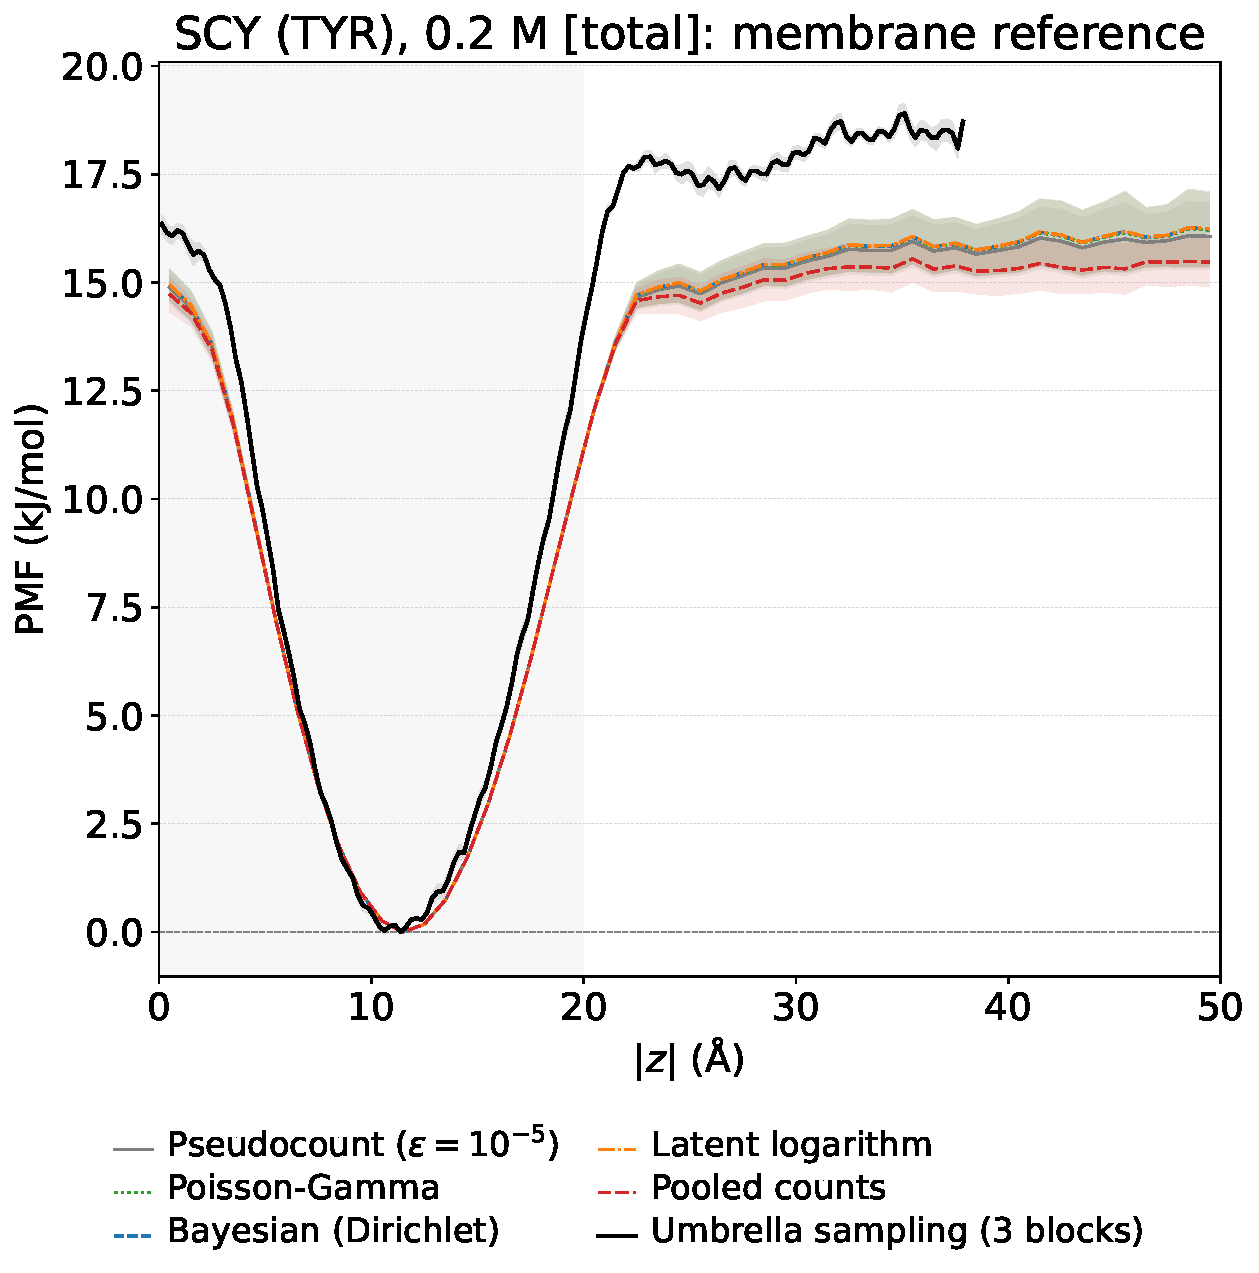
\includegraphics[width=0.49\textwidth]{FigureS_PMF_scy_methods_US_total_membrane}
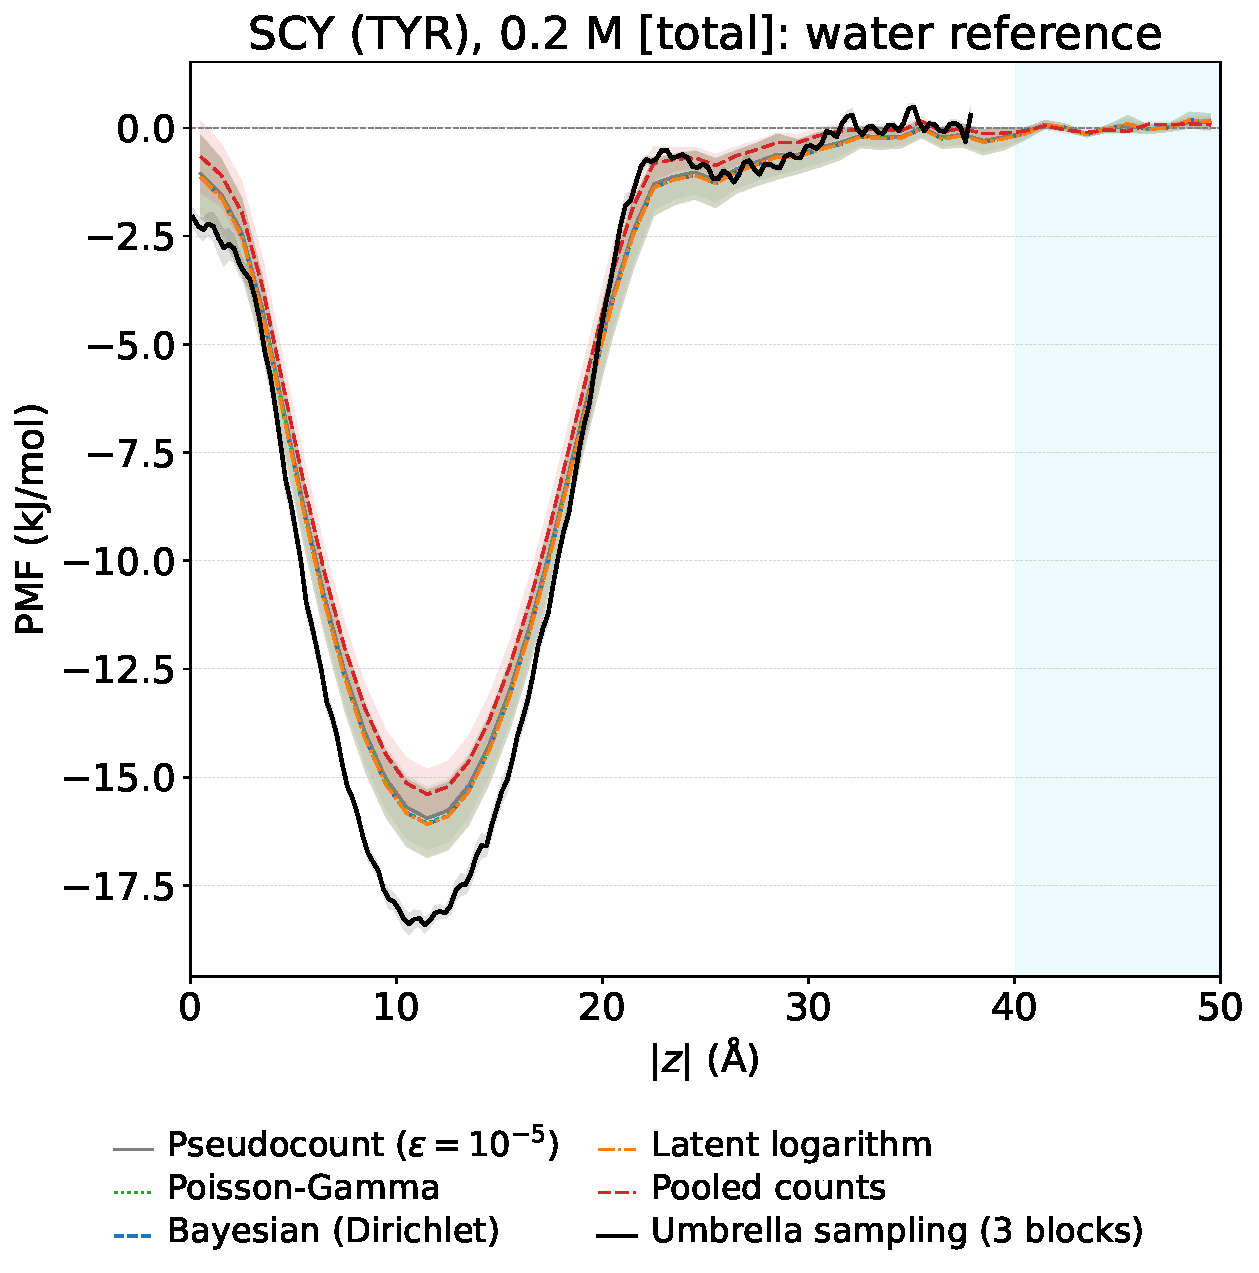
\includegraphics[width=0.49\textwidth]{FigureS_PMF_scy_methods_US_total_water}
\caption{SCY at 0.2\,M versus tyrosine US. Left: membrane reference (each minimum in
0--20\,\AA{} set to zero). Bands: untranslated SE under a fixed shift; the uncertainty of
each curve's minimum is not propagated. Right: water reference (MD: 40--50\,\AA; US: each
folded block set to zero over $|z|\ge30$\,\AA). Bands: SE. The five MD curves overlap
almost entirely; all are shallower than US in the well and have a lower bilayer-centre
barrier relative to the well (left).}
\label{fig:methods02}
\end{figure}

\begin{table}[H]
\centering
\caption{Agreement between estimators and with US (kJ\,mol$^{-1}$). ``Well'': water-referenced
minimum $\pm$ SE, at 11.5\,\AA{} for every curve (US: $-18.42 \pm 0.18$ at 11.4\,\AA).
``RMSD$_w$'': root-mean-square deviation from US with the water reference over
0--38\,\AA{} (US averaged into the 1\,\AA{} MD bins). ``RMSD$_m$'': same with the membrane
reference over 0--20\,\AA.}
\label{tab:estimators}
\small
\setlength{\tabcolsep}{5pt}
\begin{tabular}{l rrr rrr}
\toprule
 & \multicolumn{3}{c}{0.2\,M} & \multicolumn{3}{c}{0.1\,M} \\
\cmidrule(lr){2-4}\cmidrule(lr){5-7}
Estimator & Well & RMSD$_w$ & RMSD$_m$ & Well & RMSD$_w$ & RMSD$_m$ \\
\midrule
Pseudocount    & $-15.95 \pm 0.72$ & 1.30 & 1.12 & $-21.69 \pm 1.47$ & 3.03 & 0.71 \\
Poisson--Gamma & $-16.07 \pm 0.78$ & 1.24 & 1.10 & $-27.72 \pm 3.96$ & 7.84 & 0.72 \\
Bayesian       & $-16.08 \pm 0.78$ & 1.23 & 1.10 & $-24.51 \pm 2.12$ & 5.22 & 0.72 \\
Latent         & $-16.09 \pm 0.78$ & 1.23 & 1.10 & $-25.82 \pm 2.81$ & 6.25 & 0.73 \\
Pooled counts  & $-15.40 \pm 0.58$ & 1.65 & 1.15 & $-18.33 \pm 2.05$ & 0.77 & 0.71 \\
\midrule
Largest spread & \multicolumn{3}{l}{0.69 (at 12.5\,\AA)} & \multicolumn{3}{l}{9.39 (at 11.5\,\AA)} \\
\bottomrule
\end{tabular}
\end{table}

\paragraph{Why the estimators agree at 0.2\,M.} The estimators differ only in how they
handle bins with zero counts in some blocks. At 0.2\,M, every block visits water
(Table~\ref{tab:water}) and no bin between 0 and 50\,\AA{} is empty in any block, so the
pseudocount, prior, or latent model has almost nothing to fill in. The remaining spread
(0.69\kJ) is the difference between averaging logarithms and taking the logarithm of the
pooled counts, and it is smaller than the block-to-block uncertainty.

\paragraph{Remaining difference with US.} All 0.2\,M curves are 2.3--3.0\kJ{} shallower
than US in the well. With the membrane reference, they also show a lower bilayer-centre
barrier (14.7\kJ{} above the well, versus 16.4\kJ{} for US) and a lower water plateau
(15.4--15.8 versus 18.4\kJ). Because the estimators agree with each other, this difference
does not come from the treatment of zero counts.

\section{SCY at 0.1\,M}

\begin{figure}[H]
\centering
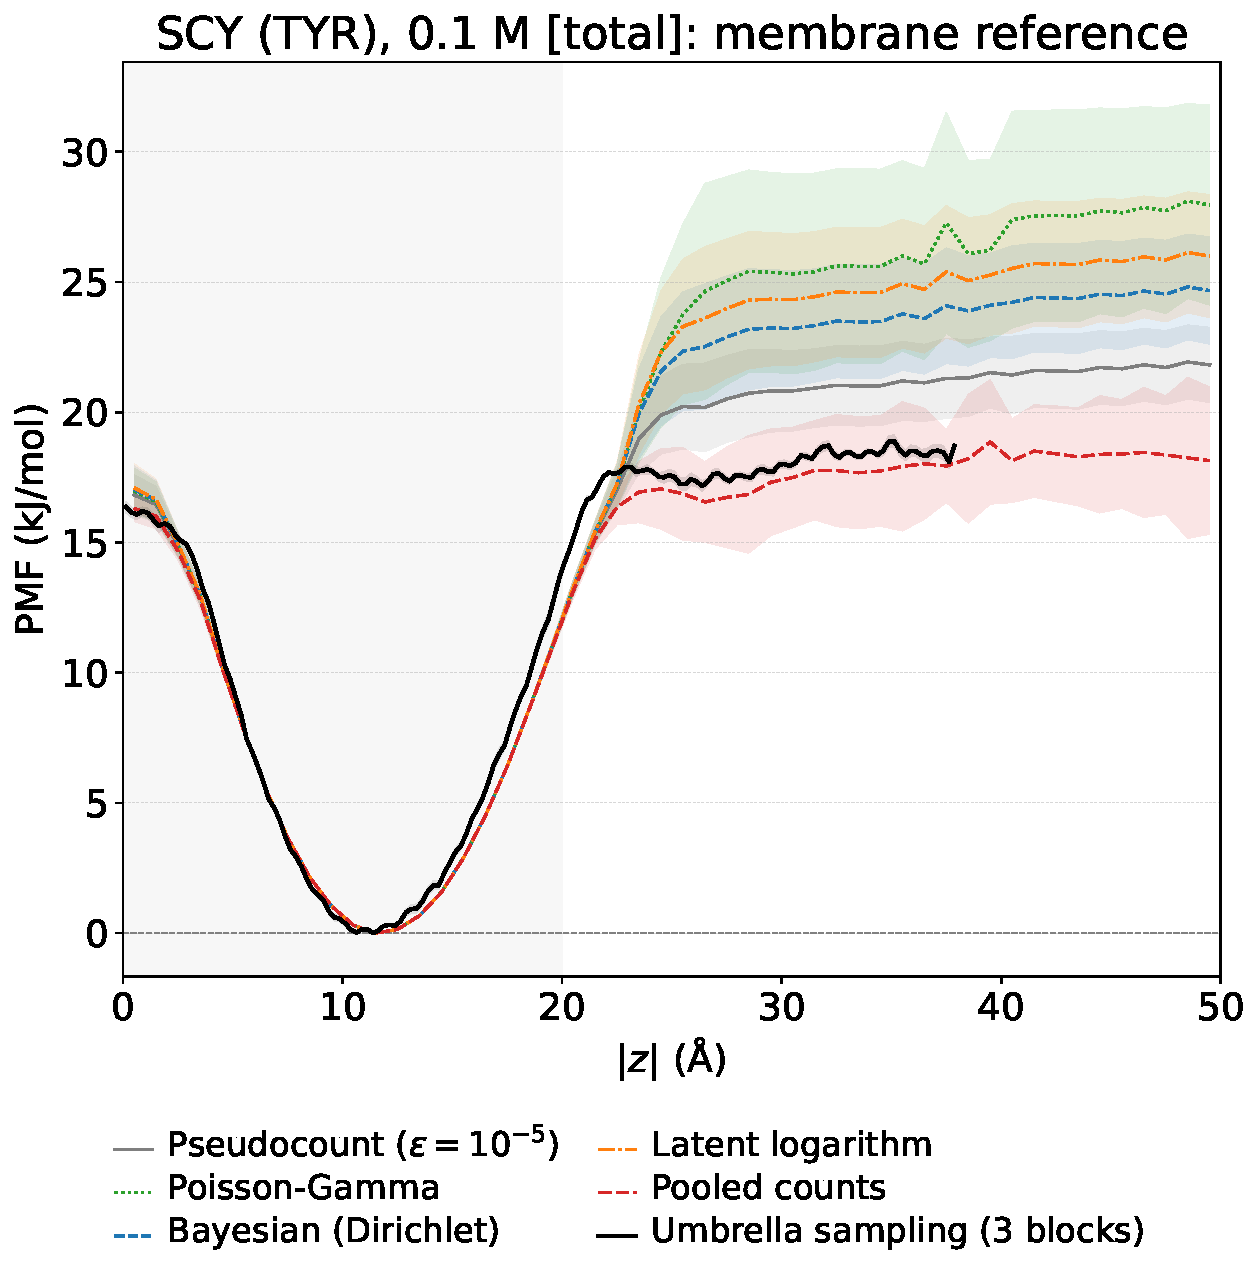
\includegraphics[width=0.49\textwidth]{FigureS_PMF_scy_01M_methods_US_total_membrane}
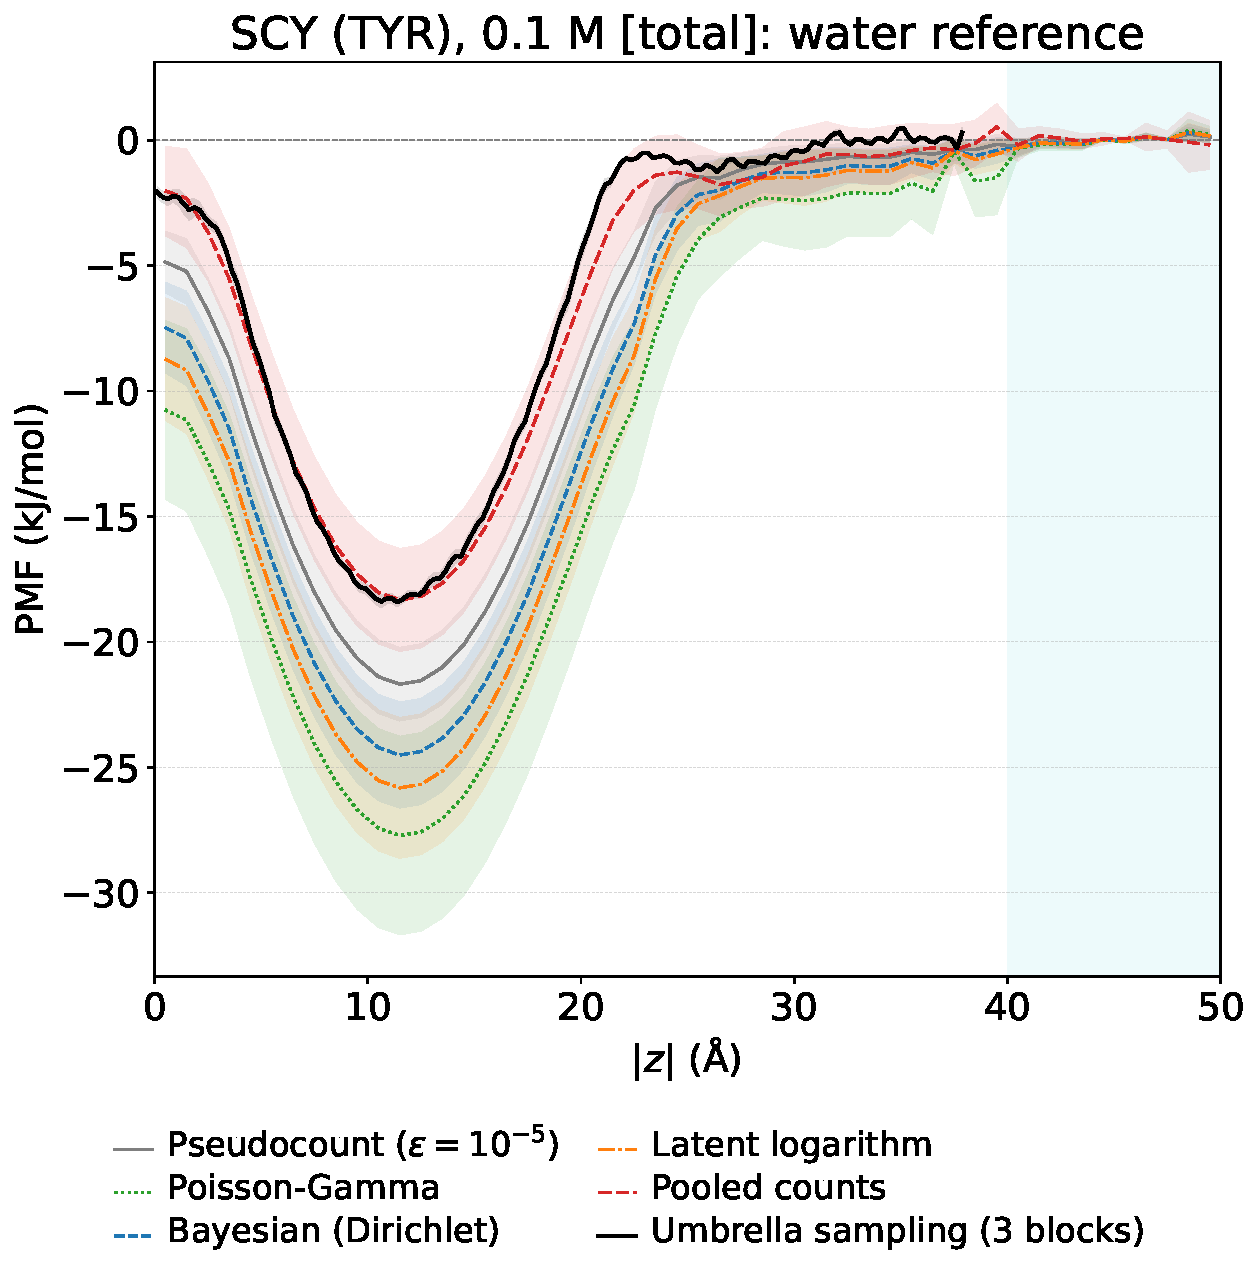
\includegraphics[width=0.49\textwidth]{FigureS_PMF_scy_01M_methods_US_total_water}
\caption{SCY at 0.1\,M versus tyrosine US. Left: membrane reference; all estimators coincide
up to about 20\,\AA, then reach water plateaus of 17.8--25.8\kJ{} (US: 18.4\kJ). Bands:
untranslated SE under a fixed shift; the uncertainty of each curve's minimum is not
propagated. Right: water reference (MD: 40--50\,\AA; US: each folded block set to zero over
$|z|\ge30$\,\AA). Only pooled counts superimpose on US. Bands: SE; the pooled-count SE excludes
bootstrap replicates without water counts (97.2\% of replicates are defined).}
\label{fig:methods01}
\end{figure}

At 0.1\,M, six of the nine blocks never reach the water window (Table~\ref{tab:water}). The
log-averaging estimators must assign a water probability to those six blocks, and the wells
then range from $-21.7$ (pseudocount) to $-27.7$\kJ{} (Poisson--Gamma). Inside the membrane,
all estimators still agree (RMSD$_m$ = 0.71--0.73\kJ{} from US). Pooled counts give
$-18.33 \pm 2.05$\kJ{} and an RMSD$_w$ of 0.77\kJ{} from US. Because the 0.1\,M water
reference comes from three blocks in two trajectories, its uncertainty is about 3.5 times
larger than at 0.2\,M ($\sigma_a = 2.05$ versus 0.57\kJ).

\begin{figure}[!htbp]
\centering
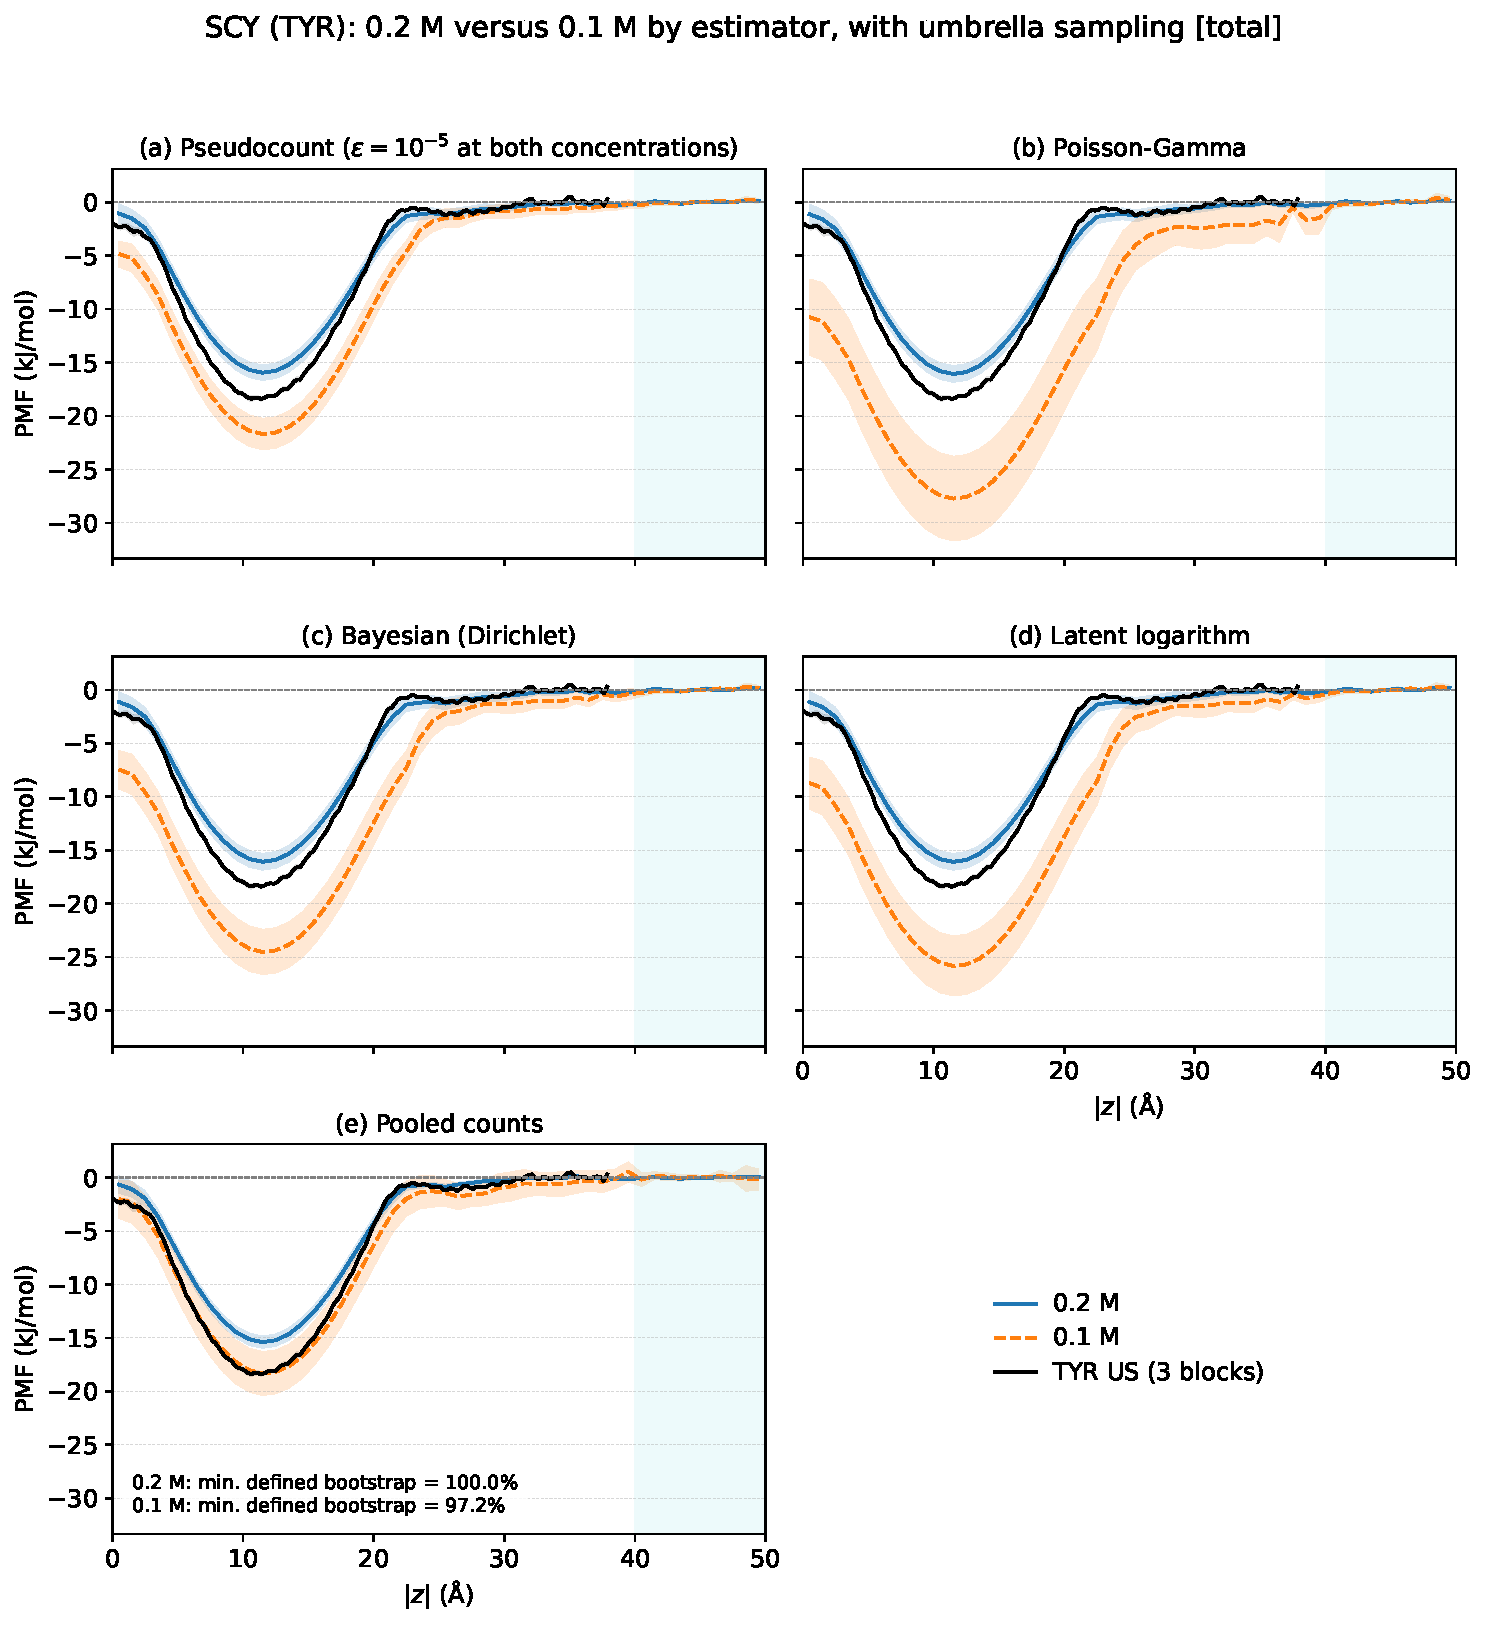
\includegraphics[width=\textwidth]{FigureS_PMF_scy_concentration_methods_US_total}
\caption{SCY at 0.2\,M versus 0.1\,M for each estimator, water reference, with tyrosine US.
For every estimator, 0.1\,M is deeper than 0.2\,M, by 2.9\kJ{} (pooled counts) to
11.7\kJ{} (Poisson--Gamma). Only the pooled-count 0.1\,M curve coincides with US. Water
references: MD 40--50\,\AA; US each folded block set to zero over $|z|\ge30$\,\AA. Bands: SE;
the pooled-count SE excludes bootstrap replicates without water counts.}
\label{fig:conc}
\end{figure}

\section{Is the concentration effect significant?}
\label{sec:pvalues}

\subsection{Test}
The test uses pooled counts, as for leucine. For each concentration, the nine blocks are
resampled independently 10\,000 times. In each replicate, the pooled PMF and its reference are
recomputed: the minimum within 0--20\,\AA{} for the membrane reference, or the mean
40--50\,\AA{} probability for the water reference. The difference
$\Delta G(z) = G_{0.2\,\text{M}}(z) - G_{0.1\,\text{M}}(z)$ is tested over 0--20\,\AA{} and
0--50\,\AA{} with two statistics:
\begin{itemize}
  \item \textbf{$p(\max|t|)$:} the largest studentised local difference, sensitive to a
  difference in any single bin;
  \item \textbf{$p(\text{offset})$:} the region-averaged difference, sensitive to a systematic
  vertical shift.
\end{itemize}
Both use the centred bootstrap null distribution; replicates with an undefined bin are
excluded. A replicate is undefined at 0.1\,M when it contains none of the three
water-visiting blocks, with probability $(6/9)^9 = 2.6\%$.

As a robustness check, the test was repeated with one 600\,ns block per trajectory (the three
200\,ns blocks of each trajectory summed), enumerating all $27 \times 27$ resample pairs.
This removes any assumption that blocks from the same trajectory are independent.

\begin{figure}[H]
\centering
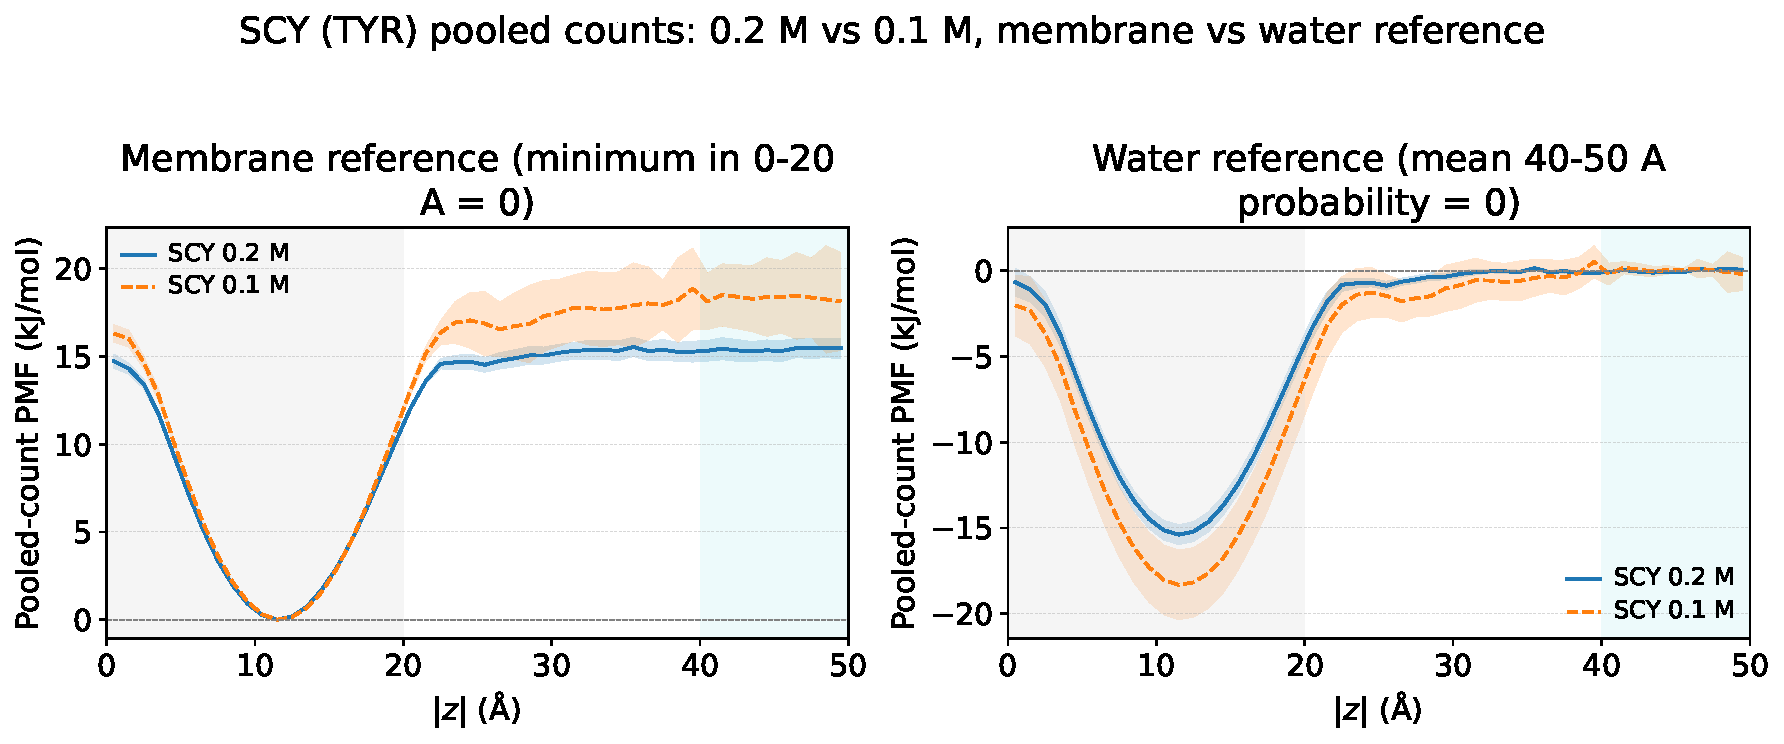
\includegraphics[width=\textwidth]{FigureS_PMF_scy_concentration_pvalues_total}
\caption{Pooled-count PMFs of SCY at 0.2 and 0.1\,M with the membrane reference (left) and the
water reference (right). Grey: 0--20\,\AA; cyan: 40--50\,\AA{} water window. Bands:
block-bootstrap SE (defined replicates only) $\times\sqrt{9/8}$, with the reference re-estimated
in every replicate. The tests of $G_{0.2\,\text{M}} - G_{0.1\,\text{M}}$ are given in
Table~\ref{tab:pvalues}.}
\label{fig:pvalues}
\end{figure}

\begin{table}[H]
\centering
\caption{Bootstrap tests of $G_{0.2\,\text{M}} - G_{0.1\,\text{M}}$ for SCY with pooled counts
(kJ\,mol$^{-1}$). Nine 200\,ns blocks; p-values: centred bootstrap, 10\,000 independent
resamples per concentration, replicates with undefined bins excluded. The last column repeats
$p(\text{offset})$ with three trajectory blocks (smallest attainable value 0.0014, reported as
an upper bound).}
\label{tab:pvalues}
\small
\setlength{\tabcolsep}{5pt}
\begin{tabular}{llrrrrrr}
\toprule
Reference & Region & Mean $\Delta G$ & Max $|\Delta G|$ & $p(\max|t|)$ & $p(\text{offset})$ & Defined & 3 traj. \\
\midrule
Membrane & 0--20\,\AA & $-0.44 \pm 0.12$ & 1.71 & 0.0010 & 0.0007 & 100.0\% & $\le 0.0014$ \\
Membrane & 0--50\,\AA & $-1.66 \pm 0.91$ & 3.58 & 0.0012 & 0.077  & 97.4\%  & $\le 0.0014$ \\
Water    & 0--20\,\AA & $+2.49 \pm 2.08$ & 3.06 & 0.126  & 0.146  & 97.4\%  & 0.087 \\
Water    & 0--50\,\AA & $+1.27 \pm 1.25$ & 3.06 & 0.093  & 0.165  & 97.4\%  & 0.117 \\
\bottomrule
\end{tabular}
\end{table}

\paragraph{Interpretation.}
\begin{itemize}
  \item \textbf{A shape difference inside the membrane.} With the membrane reference, the
  0--20\,\AA{} difference is significant with both statistics ($p \le 0.001$) and with three
  trajectory blocks ($p \le 0.0014$). It is concentrated at the bilayer centre: from
  $-1.6 \pm 0.6$\kJ{} at 0.5\,\AA{} to $-1.1 \pm 0.4$\kJ{} at 3.5\,\AA, so the 0.1\,M
  central barrier is higher (16.3 vs 14.7\kJ{} above the well). The difference is
  0.4--0.7\,$k_BT$, small but larger than for any of the aliphatic residues
  ($\le 0.11$\kJ{} on average).
  \item \textbf{No significant change in the membrane-to-water offset.} The 0.1\,M well is
  2.5--2.9\kJ{} deeper with the water reference, but $p(\text{offset}) = 0.15$--$0.17$
  (0.09--0.12 with three trajectory blocks). The membrane-referenced 0--50\,\AA{} test
  measures the same offset and gives $p = 0.077$. Its three-trajectory value
  ($p \le 0.0014$) relies on SEs estimated from only three units and should not be
  over-interpreted.
  \item \textbf{Local differences.} The small $p(\max|t|)$ values reflect the bilayer centre
  and individual interfacial bins, where 0.1\,M has few counts.
  \item \textbf{Agreement with US.} The 0.1\,M pooled-count curve matches US in the well
  (difference 0.09\kJ), at the centre barrier, and in the water plateau, whereas the 0.2\,M
  curves are about 2.5\kJ{} shallower and have a lower central barrier. A weak
  concentration effect at 0.2\,M would explain both observations, but these data do not
  establish it.
  \item \textbf{Conclusion.} Tyrosine has a reproducible concentration effect, and it is a
  change of shape at the bilayer centre (about 1.6\kJ); tryptophan shows the same effect
  (Section~\ref{sec:phe_trp}). The transfer free energy may also be about 3\kJ{} more favourable at 0.1\,M, in
  better agreement with US, but this difference is within the uncertainty of the 0.1\,M water
  reference. More 0.1\,M water-phase sampling would be needed to confirm it.
\end{itemize}

\section{Phenylalanine and tryptophan}
\label{sec:phe_trp}

The same analysis was applied to the two other aromatic residues, phenylalanine
(\texttt{scf}, \texttt{scf-1}) and tryptophan (\texttt{scw}, \texttt{scw-1}). No umbrella
sampling PMF is available for them, so only the estimators and the two concentrations can be
compared.

\begin{table}[H]
\centering
\caption{Phenylalanine and tryptophan (kJ\,mol$^{-1}$). ``Water blocks'': blocks with counts
in the 40--50\,\AA{} window (out of 9). ``Estimator wells'': range of the water-referenced
minima of the five estimators. ``Spread'': largest difference between any two estimators over
0--50\,\AA. ``Pooled well'': pooled-count minimum $\pm$ SE (at 0.5\,\AA{} for PHE and
11.5\,\AA{} for TRP).}
\label{tab:phe_trp}
\small
\setlength{\tabcolsep}{5pt}
\begin{tabular}{llcccc}
\toprule
Residue & Conc. & Water blocks & Estimator wells & Spread & Pooled well \\
\midrule
PHE & 0.2\,M & 7 & $-18.27$ to $-14.99$ & 3.3  & $-14.99 \pm 0.90$ \\
PHE & 0.1\,M & 4 & $-26.66$ to $-16.22$ & 10.4 & $-16.22 \pm 4.52$ \\
TRP & 0.2\,M & 9 & $-17.77$ to $-17.13$ & 0.6  & $-17.13 \pm 0.52$ \\
TRP & 0.1\,M & 7 & $-23.74$ to $-18.94$ & 4.8  & $-18.94 \pm 1.86$ \\
\bottomrule
\end{tabular}
\end{table}

\begin{figure}[!htbp]
\centering
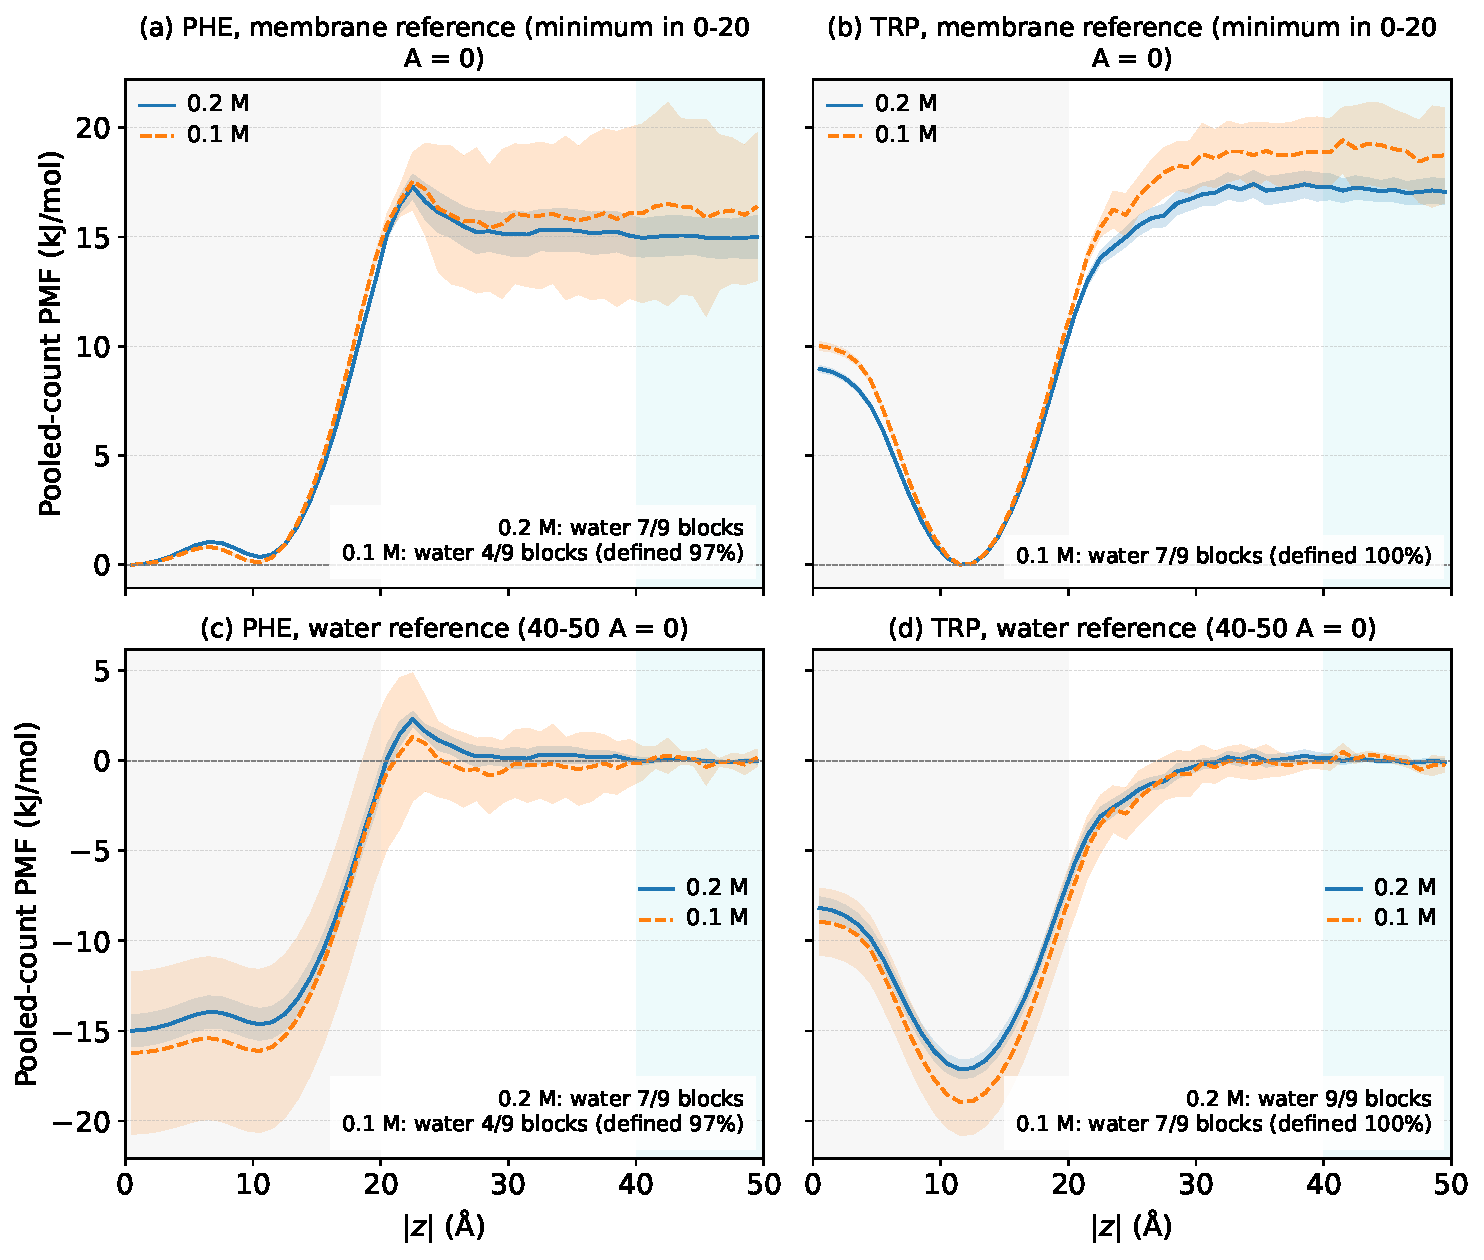
\includegraphics[width=\textwidth]{FigureS_PMF_pooled_counts_concentration_phe_trp_total}
\caption{Pooled-count PMFs of phenylalanine (left) and tryptophan (right) at 0.2 and 0.1\,M.
Top: membrane reference (each minimum in 0--20\,\AA{} set to zero). Bottom: water reference
(40--50\,\AA). Bands: block-bootstrap SE $\times\sqrt{9/8}$ (defined replicates only), with
the reference re-estimated in every replicate. Notes give the number of blocks reaching water
and, where below 100\%, the smallest fraction of defined bootstrap replicates.}
\label{fig:phe_trp}
\end{figure}

\begin{table}[H]
\centering
\caption{Bootstrap tests of $G_{0.2\,\text{M}} - G_{0.1\,\text{M}}$ for phenylalanine and
tryptophan with pooled counts (kJ\,mol$^{-1}$), as in Table~\ref{tab:pvalues}. The last column
repeats $p(\text{offset})$ with three trajectory blocks (smallest attainable value 0.0014,
reported as an upper bound).}
\label{tab:phe_trp_pvalues}
\small
\setlength{\tabcolsep}{5pt}
\begin{tabular}{lllrrrrr}
\toprule
Residue & Reference & Region & Mean $\Delta G$ & $p(\max|t|)$ & $p(\text{offset})$ & Defined & 3 traj. \\
\midrule
PHE & Membrane & 0--20\,\AA & $-0.12 \pm 0.06$ & 0.006 & 0.033 & 100.0\% & 0.10 \\
PHE & Membrane & 0--50\,\AA & $-0.51 \pm 1.94$ & 0.006 & 0.69  & 97.4\%  & 0.68 \\
PHE & Water    & 0--20\,\AA & $+1.11 \pm 4.69$ & 0.59  & 0.64  & 99.5\%  & 0.57 \\
PHE & Water    & 0--50\,\AA & $+0.73 \pm 1.95$ & 0.40  & 0.52  & 97.4\%  & 0.44 \\
\midrule
TRP & Membrane & 0--20\,\AA & $-0.55 \pm 0.07$ & 0.0001 & 0.0001 & 100.0\% & $\le 0.0014$ \\
TRP & Membrane & 0--50\,\AA & $-1.18 \pm 0.83$ & 0.0001 & 0.16   & 99.96\% & 0.12 \\
TRP & Water    & 0--20\,\AA & $+1.26 \pm 1.93$ & 0.35   & 0.46   & 100.0\% & 0.47 \\
TRP & Water    & 0--50\,\AA & $+0.63 \pm 1.13$ & 0.35   & 0.49   & 99.96\% & 0.45 \\
\bottomrule
\end{tabular}
\end{table}

\paragraph{Estimators.} Tryptophan behaves like tyrosine: at 0.2\,M every block reaches water
and the five estimators agree within 0.6\kJ. Phenylalanine is less well sampled in water
(7/9 blocks), and its estimators already differ by 3.3\kJ{} at 0.2\,M. At 0.1\,M, both
residues have blocks without water counts, and the estimators diverge by 4.8 (TRP) and
10.4\kJ{} (PHE), as for tyrosine and leucine. Pooled counts give the shallowest well in every
case.

\paragraph{Concentration.}
\begin{itemize}
  \item \textbf{Tryptophan shows the same shape change as tyrosine.} With the membrane reference,
  the 0.1\,M bilayer-centre barrier is $1.1 \pm 0.2$\kJ{} higher than at 0.2\,M (0.5--4.5\,\AA),
  relative to the interfacial well at 11.5\,\AA. The 0--20\,\AA{} offset is significant with
  nine blocks ($p = 0.0001$) and with three trajectory blocks ($p \le 0.0014$).
  \item \textbf{Phenylalanine shows only a small shape difference.} Its membrane minimum is at the
  bilayer centre, not at the interface. The 0--20\,\AA{} difference is $-0.12 \pm 0.06$\kJ{}
  on average and at most 0.9\kJ{} near 18\,\AA. It is marginal with nine blocks ($p = 0.033$)
  and not significant with three trajectory blocks ($p = 0.10$).
  \item \textbf{The membrane-to-water offset does not differ for either residue.} With the water
  reference, the 0.1\,M wells are 1.2 (PHE) and 1.8\kJ{} (TRP) deeper, with $p = 0.46$--$0.64$.
  For phenylalanine at 0.1\,M, only 4/9 blocks reach water and the well SE is 4.5\kJ, so even a
  large difference would not be detected.
\end{itemize}

\paragraph{Conclusion.} The two residues with an interfacial well, tyrosine and tryptophan, share
a reproducible concentration effect: at 0.1\,M the bilayer centre is about 1--1.6\kJ{} less
favourable relative to the well. Phenylalanine, which prefers the bilayer centre, and the
aliphatic residues show no comparable effect. No residue shows a significant change in the
membrane-to-water free energy, which is limited by the sampling of the water phase at 0.1\,M.

\section{Limitations}
\begin{itemize}
  \item Counts are molecule-frames, not independent events. Blocks within a trajectory may be
  correlated; the three-trajectory test addresses this but has a coarse null distribution.
  \item Bootstrap SEs and p-values exclude undefined replicates; at 0.1\,M they are conditional
  on drawing at least one of the three water-visiting blocks.
  \item The p-values are not corrected for multiple testing (four region/reference
  combinations, two statistics each).
  \item US uses a different water window ($\ge 30$\,\AA) and a single solute per leaflet, so it
  is not the same observable as a 0.2\,M or 0.1\,M ensemble. Agreement with US is supporting
  evidence, not proof of an unbiased estimate.
\end{itemize}

\end{document}
